% ============================================================
% 第6章：三角函数（上）——正弦与余弦的周期世界
% ============================================================

\chapter{三角函数（上）——正弦与余弦的周期世界}

\begin{applicationbox}
\textbf{学完本章你能做什么？}
\begin{enumerate}
  \item \textbf{学之前}：你学的所有函数要么增长、要么衰减——没有一个会"重复"。
  \item \textbf{学之后}：你会用 \(\sin x\) 和 \(\cos x\) 描述\textbf{周期运动}——旋转、振动、波动。
        Transformer 中的位置编码、音频信号处理、图像生成中的扩散模型，全都离不开三角函数。
  \item \textbf{日常例子}：交流电的电压随时间呈正弦变化；弹簧振子的位置随时间呈正弦变化；
        声波是空气的疏密振动——也是正弦波。
\end{enumerate}
\end{applicationbox}


% ============================================================
\section{从第5章来——一种全新的函数}
% ============================================================

前五章我们学的函数（幂、指、对）有一个共同特点：它们要么一直增长，要么一直衰减。

但现实世界中有大量\textbf{重复}的现象：
\begin{itemize}
  \item 地球绕太阳公转——每年重复一次
  \item 钟摆左右摆动——每几秒重复一次
  \item 交流电 50 赫兹——每秒重复 50 次
\end{itemize}

\textbf{周期函数}就是描述这种重复现象的数学工具，而三角函数是周期函数中最基本的。


% ============================================================
\section{弧度制——用实数度量角度}
% ============================================================

在使用三角函数之前，我们需要一种新的角度度量方式。

\begin{definitionbox}[弧度制]
\textbf{弧度}（读作 hú dù，英文 radian）是角度的另一种单位。

定义：在单位圆中，\textbf{弧长等于半径}的圆弧所对的圆心角为 \textbf{1 弧度}。

\[
1 \text{ 弧度} \approx 57.3^\circ
\]

弧度与度的换算：
\[
\pi \text{ 弧度} = 180^\circ \qquad
1 \text{ 弧度} = \frac{180^\circ}{\pi} \approx 57.3^\circ
\]
\end{definitionbox}

\begin{examplebox}[1——常见角的弧度与度数]
\begin{center}
\begin{tabular}{c|c|c}
\textbf{度数} & \textbf{弧度} & \textbf{记忆方式} \\
\hline
\(0^\circ\) & \(0\) & \\
\(30^\circ\) & \(\dfrac{\pi}{6}\) & \(180\div6 = 30\) \\
\(45^\circ\) & \(\dfrac{\pi}{4}\) & \(180\div4 = 45\) \\
\(60^\circ\) & \(\dfrac{\pi}{3}\) & \(180\div3 = 60\) \\
\(90^\circ\) & \(\dfrac{\pi}{2}\) & \(180\div2 = 90\) \\
\(180^\circ\) & \(\pi\) & \\
\(360^\circ\) & \(2\pi\) & 转一圈 \\
\end{tabular}
\end{center}

\textbf{为什么用弧度？} 因为弧度让数学公式更简洁——
\( \sin x \) 在弧度制下的导数才是 \( \cos x \)（以后学导数时会看到）。
\end{examplebox}


% ============================================================
\section{单位圆——三角函数的几何定义}
% ============================================================

\begin{definitionbox}[单位圆]
在坐标系中，以原点为圆心、半径为 1 的圆叫\textbf{单位圆}。

方程：\(x^2 + y^2 = 1\)
\end{definitionbox}

在单位圆上取一点 \(P\)，从正 \(x\) 轴逆时针旋转到 \(P\) 的角度为 \(\theta\)：

\[
\cos \theta = P \text{ 的 } x \text{ 坐标}, \qquad
\sin \theta = P \text{ 的 } y \text{ 坐标}
\]

\begin{examplebox}[2——单位圆上的 \(\sin\) 和 \(\cos\)]
\begin{center}
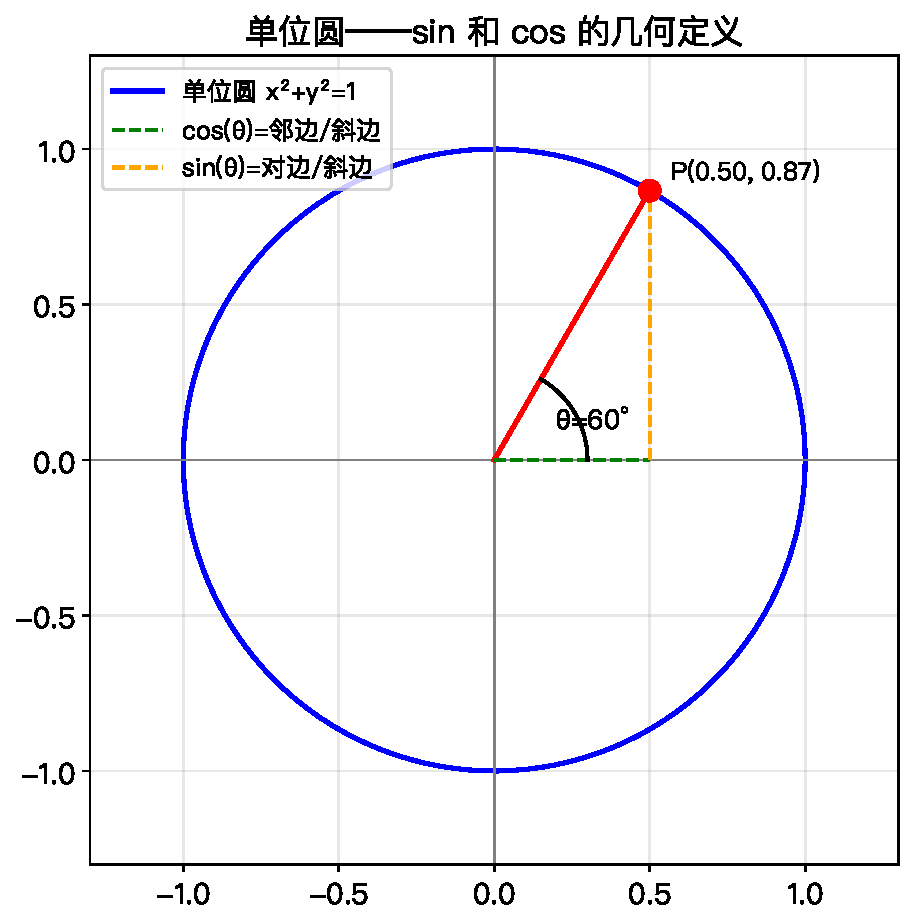
\includegraphics[width=0.5\textwidth]{figures/ch06_unit_circle.pdf}
\end{center}

以 \(\theta = 60^\circ = \dfrac{\pi}{3}\) 为例：
\[
\cos\frac{\pi}{3} = \frac{1}{2} = 0.5,\qquad
\sin\frac{\pi}{3} = \frac{\sqrt{3}}{2} \approx 0.866
\]

\textbf{验证：} \(x^2 + y^2 = (0.5)^2 + (0.866)^2 = 0.25 + 0.75 = 1\) [OK]

\textbf{关键结论：} 对任意角度 \(\theta\)：
\[
\boxed{\sin^2 \theta + \cos^2 \theta = 1}
\]
这就是\textbf{最重要的三角恒等式}。
\end{examplebox}


% ============================================================
\section{特殊角度的三角函数值}
% ============================================================

\begin{examplebox}[3——记住这几个值]
\begin{center}
\begin{tabular}{c|c|c}
\(\theta\) & \(\sin\theta\) & \(\cos\theta\) \\
\hline
\(0\) & \(0\) & \(1\) \\
\(\dfrac{\pi}{6}\) (\(30^\circ\)) & \(\dfrac{1}{2}\) & \(\dfrac{\sqrt{3}}{2}\) \\
\(\dfrac{\pi}{4}\) (\(45^\circ\)) & \(\dfrac{\sqrt{2}}{2}\) & \(\dfrac{\sqrt{2}}{2}\) \\
\(\dfrac{\pi}{3}\) (\(60^\circ\)) & \(\dfrac{\sqrt{3}}{2}\) & \(\dfrac{1}{2}\) \\
\(\dfrac{\pi}{2}\) (\(90^\circ\)) & \(1\) & \(0\) \\
\(\pi\) (\(180^\circ\)) & \(0\) & \(-1\) \\
\(\dfrac{3\pi}{2}\) (\(270^\circ\)) & \(-1\) & \(0\) \\
\(2\pi\) (\(360^\circ\)) & \(0\) & \(1\) \\
\end{tabular}
\end{center}

\textbf{记忆方法：} 从单位圆上看——
\(\sin\) 是 \(y\) 坐标（上正下负），\(\cos\) 是 \(x\) 坐标（右正左负）。
\end{examplebox}


% ============================================================
\section{正弦函数 \(y = \sin x\)}
% ============================================================

把单位圆上的 \(\sin \theta\) 值作为函数值，\(\theta\) 作为自变量，就得到正弦函数。

\begin{examplebox}[4——\(\sin x\) 的图像]
\begin{center}
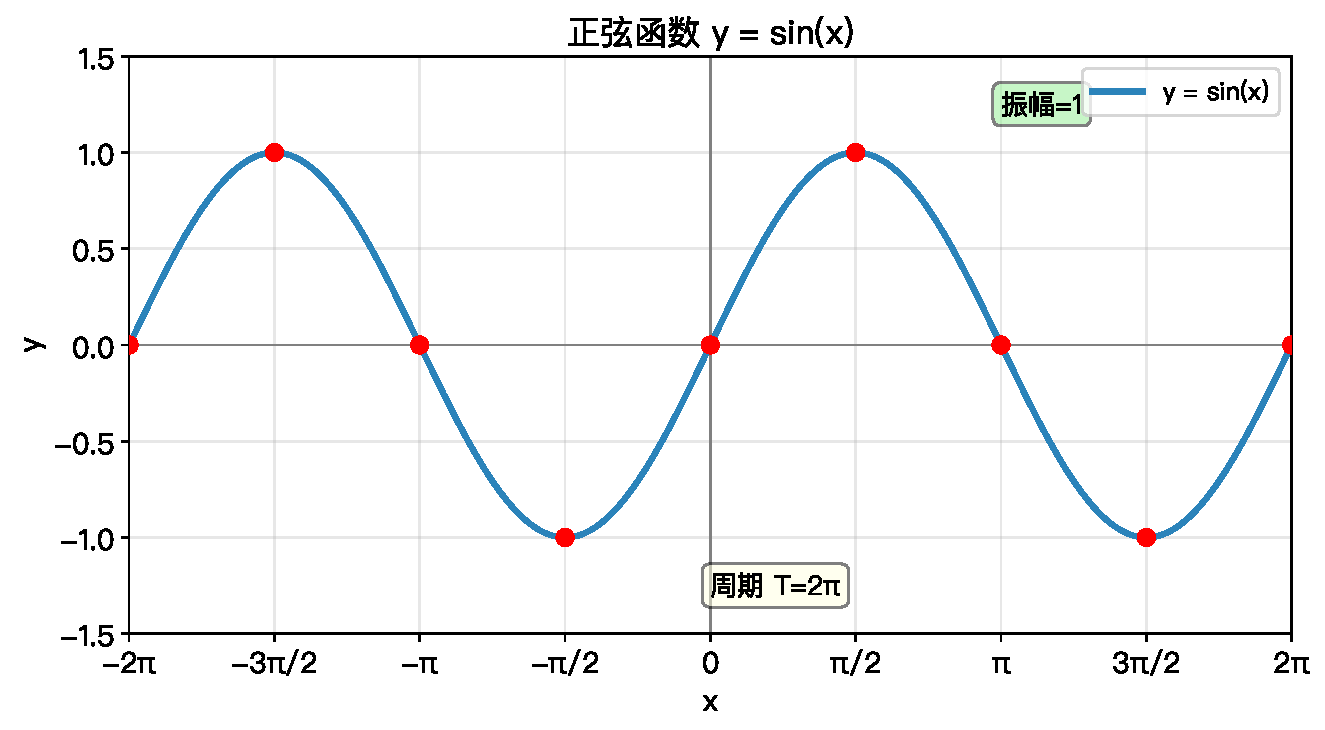
\includegraphics[width=0.85\textwidth]{figures/ch06_sine_wave.pdf}
\end{center}

\textbf{关键特征：}
\begin{enumerate}
  \item \textbf{周期性}：\(\sin(x + 2\pi) = \sin x\)——每 \(2\pi\) 重复一次
  \item \textbf{振幅}：最大值 1，最小值 \(-1\)（因为单位圆上 \(y\) 坐标在 \(-1\) 到 \(1\) 之间）
  \item \textbf{零点}：\(x = 0, \pm\pi, \pm 2\pi, \ldots\)（即 \(x = n\pi\)，\(n\) 为整数）
  \item \textbf{最大值点}：\(x = \dfrac{\pi}{2} + 2n\pi\)，\(\sin x = 1\)
  \item \textbf{最小值点}：\(x = \dfrac{3\pi}{2} + 2n\pi\)，\(\sin x = -1\)
  \item \textbf{奇函数}：\(\sin(-x) = -\sin x\)，图像关于原点对称
\end{enumerate}
\end{examplebox}

\begin{definitionbox}[正弦函数的性质]
\[
f(x) = \sin x
\]
\begin{itemize}
  \item \textbf{定义域}：\(\mathbb{R}\)（全体实数）
  \item \textbf{值域}：\([-1, 1]\)
  \item \textbf{周期}：\(T = 2\pi\)
  \item \textbf{奇偶性}：奇函数（\(\sin(-x) = -\sin x\)）
  \item \textbf{单调区间}：在 \([-\dfrac{\pi}{2}, \dfrac{\pi}{2}]\) 递增，在 \([\dfrac{\pi}{2}, \dfrac{3\pi}{2}]\) 递减
\end{itemize}
\end{definitionbox}


% ============================================================
\section{余弦函数 \(y = \cos x\)}
% ============================================================

类似地，用单位圆上的 \(x\) 坐标就得到余弦函数。

\begin{examplebox}[5——\(\cos x\) 的图像]
\begin{center}
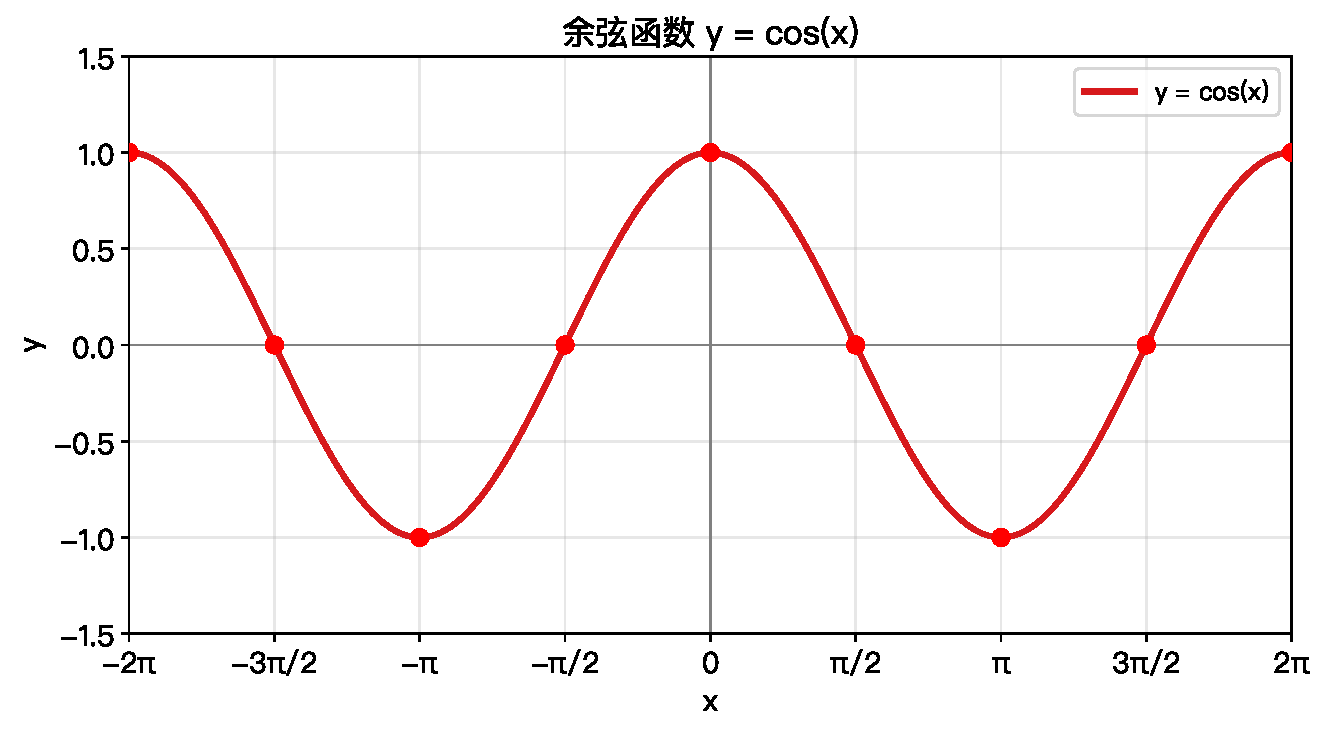
\includegraphics[width=0.85\textwidth]{figures/ch06_cosine_wave.pdf}
\end{center}

\textbf{关键特征：}
\begin{enumerate}
  \item 周期同样是 \(2\pi\)：\(\cos(x + 2\pi) = \cos x\)
  \item 值域也是 \([-1, 1]\)
  \item \textbf{偶函数}：\(\cos(-x) = \cos x\)，关于 \(y\) 轴对称
  \item \(\cos 0 = 1\)（\(\sin 0 = 0\) 的对应）
  \item 零点：\(x = \dfrac{\pi}{2} + n\pi\)
\end{enumerate}
\end{examplebox}


% ============================================================
\section{\(\sin x\) 与 \(\cos x\) 的关系}
% ============================================================

\begin{theorembox}[\(\sin\) 和 \(\cos\) 的关系]
\[
\sin\left(x + \frac{\pi}{2}\right) = \cos x, \qquad
\cos\left(x - \frac{\pi}{2}\right) = \sin x
\]

\textbf{直观理解：} \(\sin x\) 比 \(\cos x\) 领先四分之一个周期（\(\pi/2\)）。
\end{theorembox}

\begin{examplebox}[6——\(\sin\) 与 \(\cos\) 对比]
\begin{center}
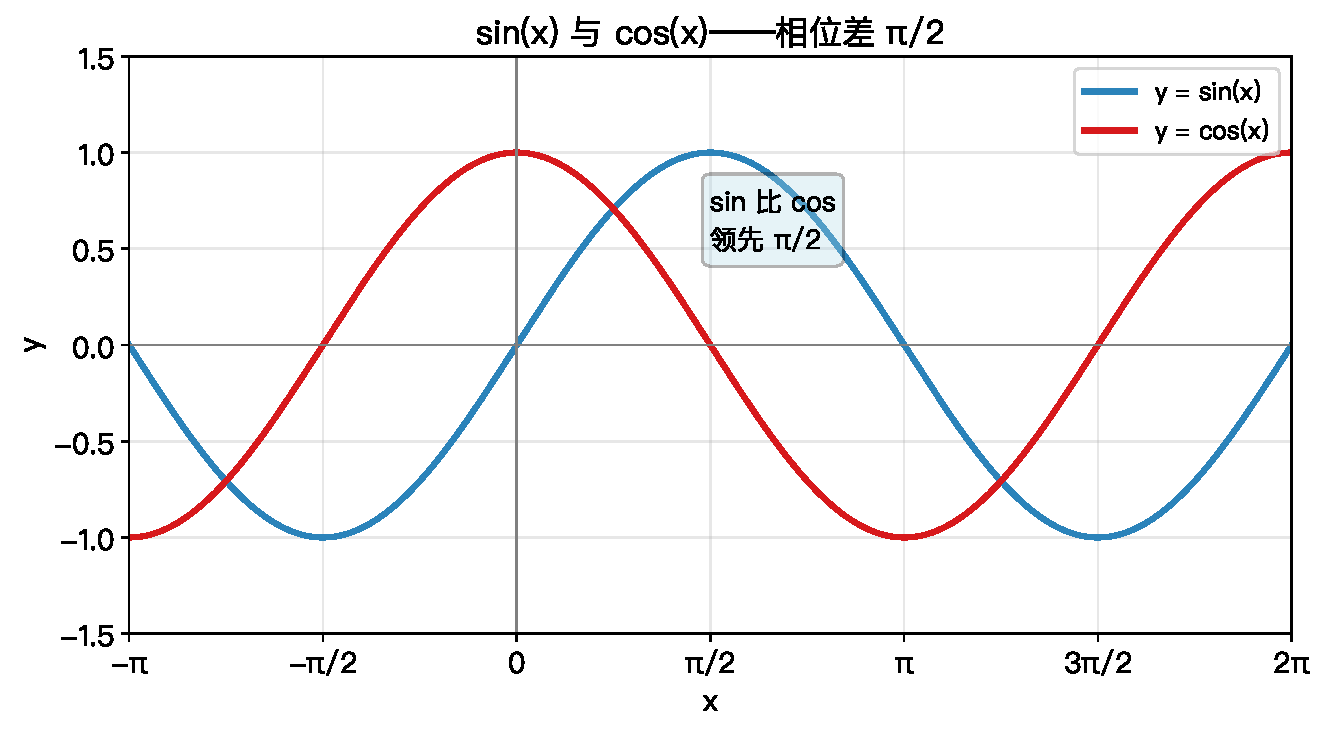
\includegraphics[width=0.85\textwidth]{figures/ch06_sine_cosine_compare.pdf}
\end{center}

\textbf{从图中可以看到：}
\begin{itemize}
  \item \(\sin x\) 在 \(x=0\) 处从 0 开始上升
  \item \(\cos x\) 在 \(x=0\) 处从 1 开始下降
  \item 把 \(\sin x\) 向左平移 \(\pi/2\) 就得到 \(\cos x\)
  \item 把 \(\cos x\) 向右平移 \(\pi/2\) 就得到 \(\sin x\)
\end{itemize}
\end{examplebox}


% ============================================================
\section{振幅与周期——控制波的形状}
% ============================================================

\begin{definitionbox}[一般形式正弦波]
\[
y = A \sin(\omega x + \varphi)
\]
其中：
\begin{itemize}
  \item \(A\) 是\textbf{振幅}——波的高度（\(|A|\)）
  \item \(\omega\) 是\textbf{角频率}——决定周期的快慢
  \item \(\varphi\) 是\textbf{初相}——决定波的起始位置
  \item \textbf{周期} \(T = \dfrac{2\pi}{\omega}\)
\end{itemize}
\end{definitionbox}

\begin{examplebox}[7——改变振幅和周期]
\begin{center}
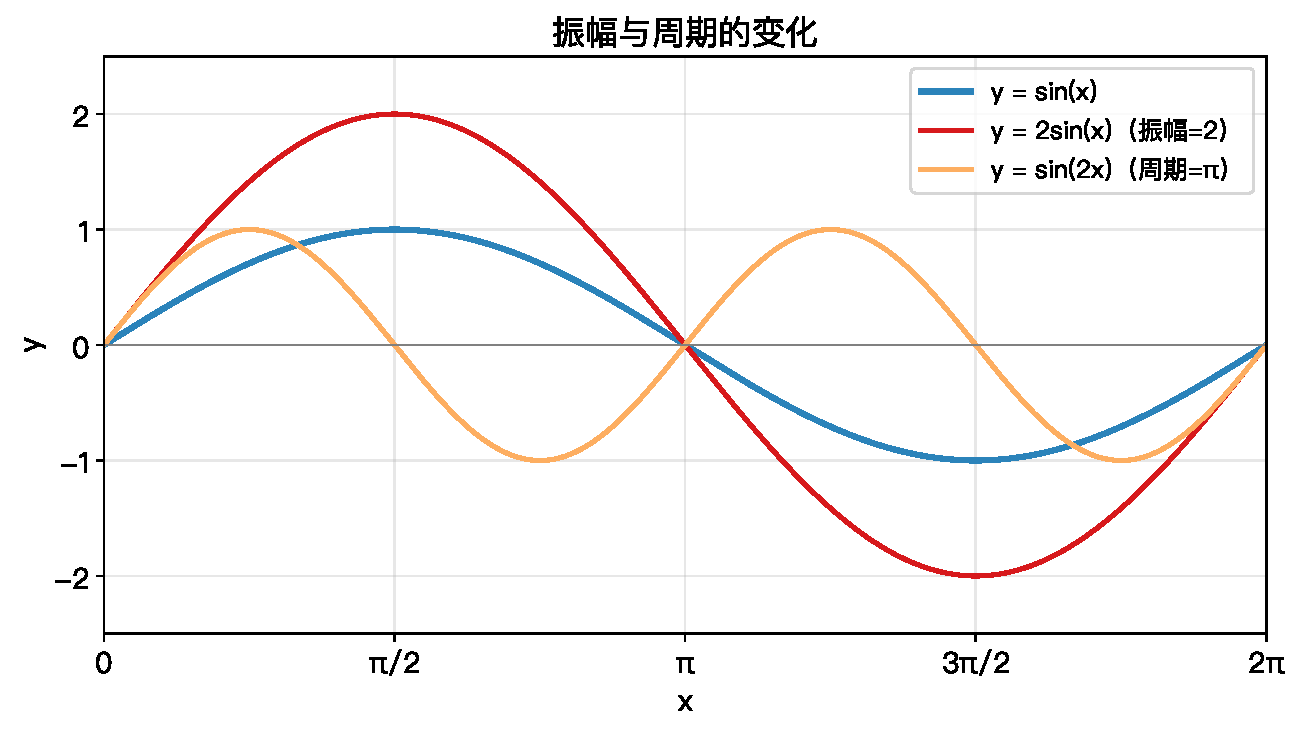
\includegraphics[width=0.85\textwidth]{figures/ch06_amplitude_period.pdf}
\end{center}

\textbf{改变振幅 \(A\)：}
\begin{itemize}
  \item \(y = \sin x\)：振幅 1，在 \(-1\) 到 \(1\) 之间
  \item \(y = 2\sin x\)：振幅 2，在 \(-2\) 到 \(2\) 之间——波更高了
\end{itemize}

\textbf{改变周期（\(\omega\)）：}
\begin{itemize}
  \item \(y = \sin x\)：周期 \(2\pi\)
  \item \(y = \sin 2x\)：周期 \(\pi\)（因为 \(T = 2\pi/2 = \pi\)）——波更密集了
\end{itemize}
\end{examplebox}


% ============================================================
\section{符号卡片}
% ============================================================

\begin{symbolcard}
\(\sin x\) & \verb|\sin x| & 读作"sin x" / "赛因 x" & 正弦函数 \\
\(\cos x\) & \verb|\cos x| & 读作"cos x" / "扣赛因 x" & 余弦函数 \\
\(\theta\) & \verb|\theta| & 读作"西塔" & 常用角度变量 \\
\(\pi\) & \verb|\pi| & 读作"派" & 圆周率，约 3.14159 \\
弧度 & —— & 读作"hú dù" & 角度的自然单位，\(180^\circ = \pi\) rad \\
周期 & —— & 读作"zhōu qī" & 函数重复一次所需的最小间隔 \\
振幅 & —— & 读作"zhèn fú" & 波峰到平衡位置的距离 \\
\end{symbolcard}


% ============================================================
\section{代码验证}
% ============================================================

\begin{lstlisting}[caption=三角函数的数值验证]
import numpy as np

# 1. 验证 sin² + cos² = 1
print("=== 验证 sin²θ + cos²θ = 1 ===")
for theta in [0, np.pi/6, np.pi/4, np.pi/3, np.pi/2, np.pi]:
    s = np.sin(theta)
    c = np.cos(theta)
    print(f"  θ={theta:5.2f}:  sin²={s**2:.6f},  cos²={c**2:.6f},  和={s**2+c**2:.6f}")

print()

# 2. 验证周期性 sin(x+2π) = sin(x)
print("=== 验证周期性 ===")
for x in [0, 0.5, 1, 2]:
    print(f"  sin({x:.1f}) = {np.sin(x):.6f},  sin({x:.1f}+2π) = {np.sin(x+2*np.pi):.6f}")

print()

# 3. 验证 sin(x+π/2) = cos(x)
print("=== 验证 sin(x+π/2) = cos(x) ===")
for x in [0, np.pi/6, np.pi/4, np.pi/3, np.pi/2]:
    lhs = np.sin(x + np.pi/2)
    rhs = np.cos(x)
    print(f"  x={x:5.2f}:  sin(x+π/2)={lhs:.6f},  cos(x)={rhs:.6f},  diff={abs(lhs-rhs):.2e}")

print()

# 4. 生成正弦波数据
print("=== 正弦波数据（前10个点）===")
x_vals = np.linspace(0, 2*np.pi, 17)  # 16等分
for x in x_vals:
    print(f"  x={x:5.2f} ({x*180/np.pi:3.0f}°):  sin={np.sin(x):7.4f},  cos={np.cos(x):7.4f}")
\end{lstlisting}

运行结果：
\begin{lstlisting}[frame=none,backgroundcolor={},numbers=none]
=== 验证 sin²θ + cos²θ = 1 ===
  θ= 0.00:  sin²=0.000000,  cos²=1.000000,  和=1.000000
  θ= 0.52:  sin²=0.250000,  cos²=0.750000,  和=1.000000
  θ= 0.79:  sin²=0.500000,  cos²=0.500000,  和=1.000000
  θ= 1.05:  sin²=0.750000,  cos²=0.250000,  和=1.000000
  θ= 1.57:  sin²=1.000000,  cos²=0.000000,  和=1.000000
  θ= 3.14:  sin²=0.000000,  cos²=1.000000,  和=1.000000
\end{lstlisting}


% ============================================================
\section{本章小结}
% ============================================================

\begin{progressbox}
\textbf{弧度制}：\(\pi\) 弧度 = \(180^\circ\)——用实数度量角度

\textbf{单位圆定义}：\(\cos\theta = x\) 坐标，\(\sin\theta = y\) 坐标

\(\sin^2 \theta + \cos^2 \theta = 1\)——最重要的三角恒等式

\textbf{正弦 }\(y = \sin x\)：周期 \(2\pi\)，值域 \([-1,1]\)，奇函数，过原点

\textbf{余弦 }\(y = \cos x\)：周期 \(2\pi\)，值域 \([-1,1]\)，偶函数，\(\cos 0 = 1\)

\textbf{相位关系}：\(\sin(x + \pi/2) = \cos x\)

\textbf{一般形式}：\(y = A \sin(\omega x + \varphi)\)，振幅 \(|A|\)，周期 \(T = 2\pi/\omega\)
\end{progressbox}

\subsection*{通往下一章}

\textbf{这一章}你学会了正弦和余弦——最基本的周期函数。

\textbf{下一章}我们继续三角函数的旅程——
正切函数、三角恒等式（和差角公式、倍角公式）、以及反三角函数。
这些是 AI 中旋转位置编码（RoPE）和傅里叶变换的基础。


% ============================================================
% 习题
% ============================================================

\section{习题}

% ===== 送分 =====

\begin{exercise}[0]
将下列度数化为弧度：
\[
(1)\; 30^\circ \qquad (2)\; 90^\circ \qquad (3)\; 180^\circ \qquad (4)\; 360^\circ
\]
\end{exercise}

\begin{exercise}[0]
求值（不用计算器）：
\[
(1)\; \sin 0 \qquad (2)\; \cos 0 \qquad (3)\; \sin \frac{\pi}{2} \qquad (4)\; \cos \pi
\]
\end{exercise}

\begin{exercise}[0]
判断正负：\(\sin 100^\circ\) 是正还是负？\(\cos 200^\circ\) 呢？
\end{exercise}

\begin{exercise}[0]
填空：\(y = \sin x\) 的周期是\_\_\_\_，值域是\_\_\_\_。
\end{exercise}

% ===== 简单 =====

\begin{exercise}[1]
求值（不用计算器，参考特殊角表格）：
\[
(1)\; \sin \frac{\pi}{6} \qquad (2)\; \cos \frac{\pi}{4} \qquad (3)\; \sin \frac{\pi}{3} \qquad (4)\; \cos \frac{\pi}{3}
\]
\end{exercise}

\begin{exercise}[1]
判断奇偶性：
\[
(1)\; y = \sin x \qquad (2)\; y = \cos x
\]
\end{exercise}

\begin{exercise}[1]
填写空白：
\[
\sin\left(x + \frac{\pi}{2}\right) = \_\_\_\_ , \qquad
\cos\left(x - \frac{\pi}{2}\right) = \_\_\_\_
\]
\end{exercise}

\begin{exercise}[1]
求 \(y = \sin x\) 在 \(x = 0, \pi/2, \pi, 3\pi/2, 2\pi\) 处的值，并画出草图。
\end{exercise}

% ===== 基础 =====

\begin{exercise}[2]
已知 \(\sin \theta = \dfrac{3}{5}\)，且 \(\theta\) 在第一象限，求 \(\cos \theta\)。
\end{exercise}

\begin{exercise}[2]
求下列函数的周期：
\[
(1)\; y = \sin 3x \qquad (2)\; y = \cos \frac{x}{2} \qquad (3)\; y = 2\sin 4x
\]
\end{exercise}

\begin{exercise}[2]
求下列函数的振幅和周期：
\[
(1)\; y = 3\sin x \qquad (2)\; y = \frac{1}{2}\cos 2x \qquad (3)\; y = -2\sin 3x
\]
\end{exercise}

\begin{exercise}[2]
判断大小（不用计算器）：
\[
(1)\; \sin 1 \text{ 和 } \cos 1 \qquad
(2)\; \sin 2 \text{ 和 } \sin 3
\]
（提示：\(\pi \approx 3.14\)，判断角度在哪个象限）
\end{exercise}

% ===== 普通 =====

\begin{exercise}[3]
化简：
\[
(1)\; \sin^2 40^\circ + \cos^2 40^\circ \qquad
(2)\; 2\sin^2 x + 2\cos^2 x \qquad
(3)\; (1 - \sin^2 x)\cos x
\]
\end{exercise}

\begin{exercise}[3]
已知 \(f(x) = 2\sin(3x)\)，求 \(f(0)\)、\(f(\pi/6)\)、\(f(\pi/2)\)。
\end{exercise}

\begin{exercise}[3]
画出 \(y = \sin x\) 和 \(y = \sin x + 1\) 在同一坐标系中的草图（一个周期即可）。
\end{exercise}

\begin{exercise}[3]
求函数 \(y = 2\cos(3x - \pi/2)\) 的：
\begin{enumerate}
  \item[(1)] 振幅
  \item[(2)] 周期
  \item[(3)] 最大值和最小值
\end{enumerate}
\end{exercise}

\begin{exercise}[3]
\(\sin 210^\circ\) 等于多少？（提示：\(210^\circ = 180^\circ + 30^\circ\)，用单位圆判断符号）
\end{exercise}

% ===== 中等 =====

\begin{exercise}[4]
证明 \(\sin(\pi - x) = \sin x\) 和 \(\cos(\pi - x) = -\cos x\)。
（提示：在单位圆上看）
\end{exercise}

\begin{exercise}[4]
解方程 \(\sin x = \dfrac{1}{2}\)，\(x \in [0, 2\pi)\)。
\end{exercise}

\begin{exercise}[4]
已知函数 \(y = 3\sin(2x - \pi/3)\)。
\begin{enumerate}
  \item[(1)] 求振幅、周期、初相
  \item[(2)] 求在 \(x=0\) 处的函数值
  \item[(3)] 这个函数是由 \(y = \sin x\) 经过怎样的变换得到的？
\end{enumerate}
\end{exercise}

\begin{exercise}[4]
弹簧振子的位移 \(d(t) = 5\cos(2\pi t)\)，其中 \(t\) 是时间（秒）。
\begin{enumerate}
  \item[(1)] 求振幅和周期
  \item[(2)] \(t=0\) 时位移是多少？
  \item[(3)] 什么时刻位移为 0？
\end{enumerate}
\end{exercise}

\begin{exercise}[4]
验证 \(\sin(x + \pi) = -\sin x\) 和 \(\cos(x + \pi) = -\cos x\)，
并用这个性质解释为什么 \(\sin x\) 和 \(\cos x\) 的周期是 \(2\pi\)。
\end{exercise}

% ===== 进阶 =====

\begin{exercise}[5]
求函数 \(y = \sin x + \sqrt{3}\cos x\) 的最大值。
（提示：利用公式 \(a\sin x + b\cos x = \sqrt{a^2 + b^2}\sin(x + \varphi)\)）
\end{exercise}

\begin{exercise}[5]
已知 \(\sin^2 \theta + \cos \theta = 1\)，且 \(0 \le \theta \le 2\pi\)，求 \(\theta\)。
\end{exercise}

\begin{exercise}[5]
一个交流电压 \(V(t) = 220\sin(100\pi t)\)（\(t\) 为秒）。
\begin{enumerate}
  \item[(1)] 求电压的周期和频率（频率 = 1/周期）
  \item[(2)] 求电压的最大值
  \item[(3)] 在 \(t = 0.005\) 秒时电压是多少？
\end{enumerate}
\end{exercise}

\begin{exercise}[5]
已知 \(f(x) = \sin x + \cos x\)。
\begin{enumerate}
  \item[(1)] 求 \(f(x)\) 的最大值和最小值
  \item[(2)] 求 \(f(x)\) 的周期
\end{enumerate}
\end{exercise}

% ===== 拔高 =====

\begin{exercise}[6]
已知 \(\sin \theta + \cos \theta = \dfrac{1}{2}\)，求：
\[
(1)\; \sin \theta \cos \theta \qquad (2)\; \sin^3 \theta + \cos^3 \theta
\]
（提示：利用 \((\sin\theta + \cos\theta)^2 = 1 + 2\sin\theta\cos\theta\)）
\end{exercise}

\begin{exercise}[6]
函数 \(y = \sin x\) 的图像经过以下变换，写出新函数的表达式：
\[
y = \sin x \xrightarrow{\text{纵坐标伸长为2倍}} \xrightarrow{\text{横坐标压缩为1/3}} \xrightarrow{\text{向右平移 }\pi/4}
\]
\end{exercise}

\begin{exercise}[6]
求证 \(\dfrac{1 - 2\sin^2 x}{\cos x + \sin x} = \cos x - \sin x\)。
\end{exercise}

% ===== 极难 =====

\begin{exercise}[7]
已知 \(f(x) = |\sin x| + |\cos x|\)。
\begin{enumerate}
  \item[(1)] 求 \(f(x)\) 的周期（提示：画图或用数值试探）
  \item[(2)] 求 \(f(x)\) 的值域
  \item[(3)] 验证：\([f(x)]^2 = 1 + |\sin 2x|\)
\end{enumerate}

\textbf{说明：} 这道题结合了绝对值、三角函数和周期，需要画图辅助思考。
绝对值函数的周期往往比原函数更短——这是一个重要的观察。
\end{exercise}
